\problem{Robot Motion}

\noindent
UVa 10116\bigskip

A robot has been programmed to follow the instructions in its path.
 Instructions for the next
direction the robot is to move are laid down in a grid.  The possible
instructions are

\begin{description}
    \item[N] north (up the page)
    \item[S] south (down the page)
    \item[E] east (to the right on the page)
    \item[W] west (to the left on the page)
\end{description}

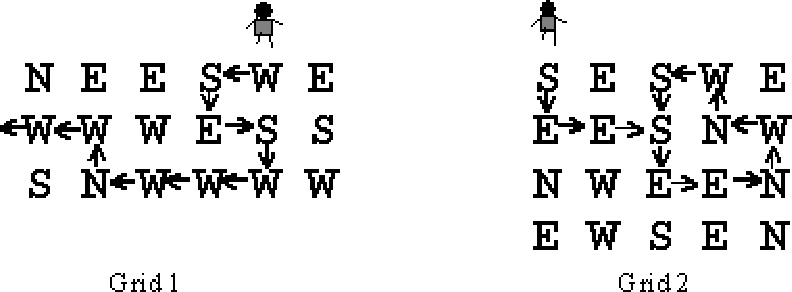
\includegraphics[width=12cm]{problems/p10116.pdf}

For example, suppose the robot starts on the north (top) side of Grid 1
and starts
south (down).  The path the robot follows is shown.  The robot goes through 
10 instructions
in the grid before leaving the grid.

Compare what happens in Grid 2:  the robot goes through 3  instructions
only once, and then
starts a loop through 8 instructions, and never exits.

You are to write a program that determines how long it takes a robot to get out of the grid or
how the robot loops around.



\subsection*{The Input}

There will be one or more grids for robots to navigate.  The data for
each is in the following form. On the first line are three integers
separated by blanks:  the number of rows in the grid, the number of
columns in the grid, and the number of the column in which the robot
enters from the north.  The possible entry columns are numbered starting
with one at the left.  Then come the rows of the direction instructions.
Each grid will have at least one and at most 10 rows and columns
of instructions.  The lines of instructions contain only the characters
N,S,E or W
with no blanks.

The end of  input is indicated by a row containing 0 0 0.
 
\subsection*{The Output}

For each grid in the input there is one line of output.  Either the robot
follows a certain
number of  instructions and exits the grid on any one the four sides or
else the robot follows
the instructions on a certain number of locations once, and then the
instructions on some
number of locations repeatedly. The sample input below corresponds to the
two grids above
and illustrates the two forms of output.  
The word "step" is
always
immediately followed by "(s)" whether or not the number before it is 1.

\subsection*{Sample Input}
\begin{verbatim}
3 6 5
NEESWE
WWWESS
SNWWWW
4 5 1
SESWE
EESNW
NWEEN
EWSEN
0 0 0    
\end{verbatim}

\subsection*{Sample Output}
\begin{verbatim}
10 step(s) to exit
3 step(s) before a loop of 8 step(s) 
\end{verbatim}

